%%% Local Variables:
%%% mode: latex
%%% TeX-master: t
%%% End:

\documentclass{article}

%%% Package imports
\usepackage[utf8]{inputenc}
\usepackage[ruled]{algorithm2e}
\usepackage{hyperref}
\usepackage{amsmath}
\usepackage{zed-csp}
\usepackage{breqn}
\usepackage{xcolor}
\usepackage{listings}
\usepackage{pgfplots}
\usepgfplotslibrary{dateplot}
\usetikzlibrary{pgfplots.dateplot}
\usepackage{pgfplotstable}

\lstset{literate = {-}{-}1} % get dashs to show up

%%% https://tex.stackexchange.com/questions/195486/how-can-i-highlight-json-string-values-but-not-attributes/195540#195540
%%% ^ JSON style for lstset
\newcommand\JSONnumbervaluestyle{\color{blue}}
\newcommand\JSONstringvaluestyle{\color{red}}
\newif\ifcolonfoundonthisline
\makeatletter

\lstdefinestyle{json}
{
  showstringspaces    = false,
  keywords            = {false,true},
  alsoletter          = 0123456789.,
  morestring          = [s]{"}{"},
  stringstyle         = \ifcolonfoundonthisline\JSONstringvaluestyle\fi,
  MoreSelectCharTable =%
  \lst@DefSaveDef{`:}\colon@json{\processColon@json},
  basicstyle          = \ttfamily,
  keywordstyle        = \ttfamily\bfseries,
}

\newcommand\processColon@json{%
  \colon@json%
  \ifnum\lst@mode=\lst@Pmode%
  \global\colonfoundonthislinetrue%
  \fi
}

\lst@AddToHook{Output}{%
  \ifcolonfoundonthisline%
  \ifnum\lst@mode=\lst@Pmode%
  \def\lst@thestyle{\JSONnumbervaluestyle}%
  \fi
  \fi
  % override by keyword style if a keyword is detected!
  \lsthk@DetectKeywords%
}

% reset the switch at the end of line
\lst@AddToHook{EOL}%
{\global\colonfoundonthislinefalse}

\makeatother
\pgfplotsset{compat=1.16}

\title{DAVE Framework: Learning Analytics Algorithms}
\author{Yet Analytics}

\begin{document}

\begin{titlepage}
  \maketitle
\end{titlepage}

\section*{Introduction}
This document introduces the initial learning analytics algorithms,
\textbf{timeline of learner success} and \textbf{which assessment
  questions are the most difficult}  of the DAVE framework.
This document will be updated to include the remaining learning analytics questions defined within the
\href{https://adloffice365.sharepoint.com/sites/TLA_Extranet/Shared\%20Documents/2018\%20TLA\%20Data\%20Requirements\%20Aligned\%20to\%20Event.docx?d=w1cf1d6fe161b4606a11c130baae5f5e1}{2018 TLA Data Requirements}
document in addition to other learning analytics algorithms which have
yet to be defined. Updates may also address refinment of these
algorithms and this document should be understood to be an example of
algorithm presentation and not the final state of any defined algorithm.
$\\\\$
The structure of this documents is as follows:
\begin{enumerate}
\item A formal specification for the data standard xAPI written in Z
  and referenced within the formal specifications of learning
  analytics algorithms
\item An algorithm definition which will consist of:
  \begin{enumerate}
  \item an introduction for the algorithm
  \item the structure of the ideal input data
  \item how to retrieve input data from an LRS
  \item the statement parameters which the algorithm will utilize
  \item any issues with the data collected during the 2018 pilot test of
    the TLA
  \item a summary of the algorithm
  \item the formal specification of the algorithm
  \item pseudocode representation of the algorithm
  \item JSONSchema for the output of the algorithm
  \item a description of the associated visualization
  \item a prototype of the visualization
  \item a collection of suggestions describing how the algorithm could be
    adapted to improve the quality of the visualization prototype
  \end{enumerate}
\end{enumerate}
$\\\\\\\\\\\\$ %%% only introduction on the first page
\section{xAPI Formal Specification}
The current formal specification only defines xAPI statements
abstractly within the context of Z. A concrete definition for xAPI
statements it outside the scope of this document.

\subsection{Basic Types}
$IFI$ ::=$ mbox \,|\, mbox\_sha1sum \,|\, openid \,|\, account$
\begin{itemize}
\item Type unique to Agents and Groups, The concrete definition of the listed values
  is outside the scope of this specification
\end{itemize}
$OBJECTTYPE$ ::=$ Agent \,|\, Group \,|\, SubStatement \,|\,
StatementRef \,|\, Activity$
\begin{itemize}
\item A type which can be present in all activities as defined by
  the xAPI specification
\end{itemize}
$INTERACTIONTYPE$ ::= $true-false \,|\, choice \,|\, fill-in \,|\,
long-fill-in \,|\, matching \,| \\ performance \,|\, sequencing \,|\,
likert \,|\, numeric \,|\, other$
\begin{itemize}
\item A type which represents the possible interactionTypes as
  defined within the xAPI specification
\end{itemize}
$INTERACTIONCOMPONENT$ ::= $choices \,|\, scale \,|\, source \,|\,
target \,|\, steps$
\begin{itemize}
\item A type which represents the possible interaction components as
  defined within the xAPI specification
\item the concrete definition of the listed values is outside the
  scope of this specification
\end{itemize}
$CONTEXTTYPES$ ::= $parent \,|\, grouping \,|\, category \,|\, other$
\begin{itemize}
\item A type which represents the possible context types as
  defined within the xAPI specification
\end{itemize}
$[STATEMENT]$
\begin{itemize}
\item Basic type for an xAPI data point
\end{itemize}
$[AGENT, GROUP]$
\begin{itemize}
\item Basic types for Agents and collections of Agents
\end{itemize}

\subsection{Id Schema}
\begin{schema}{Id}
  id : \finset_1 \#1
\end{schema}
\begin{itemize}
\item the schema $Id$ introduces the component $id$ which is a
  non-empty, finite set of 1 value
\end{itemize}

\subsection{Schemas for Agents, Groups and Actors}

\begin{schema}{Agent}
  agent : AGENT \\
  objectType : OBJECTTYPE \\
  name : \finset_1 \#1 \\
  ifi : IFI
  \where
  objectType = Agent \\
  agent = \{ifi\} \cup \power \{name, objectType\}
\end{schema}
\begin{itemize}
\item The schema $Agent$ introduces the component $agent$ which is a set
  consisting of an $ifi$ and optionally an $objectType$ and/or $name$
\end{itemize}

\begin{schema}{Member}
  Agent \\
  member : \finset_1
  \where
  member = \{a : AGENT \,|\, \forall a: a_{0}..a_{n} @ a = agent\}
\end{schema}
\begin{itemize}
\item The schema $Member$ introduces the component $member$ which is a set of
  objects $a$, where for every $a$ within $a_{0}..a_{n}$, $a$ is an $agent$
\end{itemize}

\begin{schema}{Group}
  Member \\
  group : GROUP \\
  objectType : OBJECTTYPE \\
  ifi : IFI\\
  name : \finset_1 \#1
  \where
  objectType = Group \\
  group = \{objectType, name, member\} \lor \{objectType, member\}
  \lor \\ \t2 \{objectType, ifi\} \cup \power \{name, member\}
\end{schema}
\begin{itemize}
\item The schema $Group$ introduces the component $group$ which is of
  type $GROUP$ and is a set of either $objectType$ and $member$ with optionaly $name$ or
  $objectType$ and $ifi$ with optionally $name$ and/or $member$
\end{itemize}

\begin{schema}{Actor}
  Agent \\
  Group \\
  actor : AGENT \lor GROUP
  \where
  actor = agent \lor group
\end{schema}
\begin{itemize}
\item The schema $Actor$ introduces the component $actor$ which
  is either an $agent$ or $group$
\end{itemize}

\subsection{Verb Schema}
\begin{schema}{Verb}
  Id \\
  display, verb : \finset_1
  \where
  verb = \{id, display\} \lor \{id\}
\end{schema}
\begin{itemize}
\item The schema $Verb$ introduces the component $verb$ which
  is a set that consists of either $id$ and the non-empty, finite set
  $display$ or just $id$
\end{itemize}

\subsection{Object Schema}

\begin{schema}{Extensions}
  extensions, extensionVal : \finset_1 \\
  extensionId : \finset_1 \#1 \\
  \where
  extensions = \{e : (extensionId, extensionVal)\ \,|\,
  \forall e : e_{i}..e_{j} @ \\
  \t3 \, (extensionId_{i}, extensionVal_{i})
  \lor (extensionId_{i}, extensionVal_{j}) \land \\
  \t3 \, (extensionId_{j}, extensionVal_{i})
  \lor (extensionId_{j}, extensionVal_{j})
  \land \\ \t3 \, extensionId_{i} \not = extensionId_{j}\}
\end{schema}
\begin{itemize}
\item The schema $Extensions$ introduces the component $extensions$ which
  is a non-empty, finite set that consists of ordered pairs of
  $extensionId$ and $extensionVal$. Different $extensionId$s can
  have the same $extensionVal$ but there can not be two identical
  $extensionId$ values
\item $extensionId$ is a non-empty, finite set with one value
\item $extensionVal$ is a non-empty, finite set
\end{itemize}

\begin{schema}{InteractionActivity}
  interactionType : INTERACTIONTYPE \\
  correctResponsePattern : \seq_1 \\
  interactionComponent: INTERACTIONCOMPONENT \\
  \where
  interactionActivity = \{interactionType, correctReponsePattern,
  interactionComponent\} \lor \\ \t5 \{interactionType, correctResponsePattern\}
\end{schema}
\begin{itemize}
\item The schema $InteractionActivity$ introduces the component
  $interactionActivity$ which is a set of either $interactionType$
  and $correctResponsePattern$ or $interactionType$ and
  $correctResponsePattern$ and $interactionComponent$
\end{itemize}

\begin{schema}{Definition}
  InteractionActivity \\
  Extensions \\
  definition, name, description : \finset_1 \\
  type, moreInfo : \finset_1 \#1
  \where
  definition = \power_1 \{name, description, type, moreInfo,
  extensions, interactionActivity\} \\
\end{schema}
\begin{itemize}
\item The schema $Definition$ introduces the component
  $definition$ which is the non-empty, finite power set of $name$, $description$,
  $type$, $moreInfo$ and $extensions$
\end{itemize}

\begin{schema}{Object}
  Id \\
  Definition \\
  Agent \\
  Group \\
  Statement \\
  objectTypeA, objectTypeS, objectTypeSub, objectType  : OBJECTTYPE \\
  substatement : STATEMENT \\
  object : \finset_1 \\
  \where
  substatement = statement \\
  objectTypeA = Activity \\
  objectTypeS = StatementRef \\
  objectTypeSub = SubStatement \\
  objectType = objectTypeA \lor objectTypeS \\
  object = \{id\} \lor \{id, objectType\} \lor \{id, objectTypeA,
  definition\} \\ \t2 \lor \{id, definition\} \lor \{agent\} \lor
  \{group\} \lor \{objectTypeSub, substatement\} \\
  \t2 \lor \{id, objectTypeA\}
\end{schema}
\begin{itemize}
\item The schema $Object$ introduces the component $object$ which
  is a non-empty, finite set of either $id$, $id$ and $objectType$,
  $id$ and $objectTypeA$, $id$ and $objectTypeA$ and $definition$,
  $agent$, $group$, or $substatement$
\item The schema $Statement$ and the corresponding component
  $statement$ will be defined later on in this specification
\end{itemize}
$\\\\\\\\\\\\$ %%% Header with content
\subsection{Result Schema}

\begin{schema}{Score}
  score : \finset_1 \\
  scaled, min, max, raw : \num \\
  \where
  scaled = \{ n : \num \,|\, -1.0 \leq n \leq 1.0 \} \\
  min = n < max \\
  max = n > min \\
  raw = \{ n : \num \,|\, min \leq n \leq max \} \\
  score = \power_1 \{scaled, raw, min, max\}
\end{schema}
\begin{itemize}
\item The schema $Score$ introduces the component $score$ which is
  the non-empty powerset of $min$, $max$, $raw$ and $scaled$
\end{itemize}

\begin{schema}{Result}
  Score \\
  Extensions \\
  success, completion, response, duration : \finset_1 \#1 \\
  result : \finset_1
  \where
  success = \{true\} \lor \{false\} \\
  completion = \{true\} \lor \{false\} \\
  result = \power_1 \{score, success, completion, response,
  duration, extensions\}
\end{schema}
\begin{itemize}
\item The schema $Result$ introduces the component $result$ which is
  the non-empty power set of $score$, $success$, $completion$,
  $response$, $duration$ and $extensions$
\end{itemize}

\subsection{Context Schema}

\begin{schema}{Instructor}
  Agent \\
  Group \\
  instructor : AGENT \lor GROUP
  \where
  instructor = agent \lor group
\end{schema}
\begin{itemize}
\item The schema $Instructor$ introduces the component $instructor$
  which can be ether an $agent$ or a $group$
\end{itemize}

\begin{schema}{Team}
  Group \\
  team : GROUP
  \where
  team = group
\end{schema}
\begin{itemize}
\item The schema $Team$ introduces the component $team$ which is a $group$
\end{itemize}

\begin{schema}{Context}
  Instructor \\
  Team \\
  Object \\
  Extensions \\
  registration, revision, platform, language : \finset_1 \#1 \\
  parentT, groupingT, categoryT, otherT : CONTEXTTYPES \\
  contextActivities, statement : \finset_1
  \where
  statement = object \hide (id, objectType, agent, group,
  definition) \\
  parentT = parent \\
  groupingT = grouping \\
  categoryT = category \\
  otherT = other \\
  contextActivity = \{ca : object \hide (agent, group, objectType,
  objectTypeSub, substatement)\} \\
  contextActivityParent = (parentT, contextActivity) \\
  contextActivityCategory = (categoryT, contextActivity) \\
  contextActivityGrouping = (groupingT, contextActivity) \\
  contextActivityOther = (otherT, contextActivity) \\
  contextActivities = \power_1 \{contextActivityParent,
  contextActivityCategory, \\ \t5 \:\: contextActivityGrouping,
  contextActivityOther\} \\
  context = \power_1 \{registration, instructor, team,
  contextActivities, revision, \\ \t3 platform, language, statement, extensions\}
\end{schema}
\begin{itemize}
\item The schema $Context$ introduces the component $context$
  which is the non-empty powerset of $registration$, $instructor$,
  $team$, $contextActivities$, $revision$, $platform$, $language$,
  $statement$ and $extensions$
\item The notation $object \hide agent$ represents the component
  $object$ except for its subcomponent $agent$
\end{itemize}

\subsection{Timestamp and Stored Schema}

\begin{schema}{Timestamp}
  timestamp : \finset_1 \#1
\end{schema}

\begin{schema}{Stored}
  stored : \finset_1 \#1
\end{schema}
\begin{itemize}
\item The schema $Timestamp$ and $stored$ introduce the components
  $timestamp$ and $stored$ respectively. Each are non-empty, finite
  sets containing one value
\end{itemize}
$\\ \\$
\subsection{Attachements Schema}

\begin{schema}{Attachments}
  display, description, attachment, attachments: \finset_1 \\
  usageType, sha2, fileUrl, contexntType : \finset_1 \#1 \\
  length : \nat
  \where
  attachment = \{usageType, display, contentType, length, sha2 \}
  \cup \power \{description, fileUrl\} \\
  attachments = \{a : attachment\}
\end{schema}
\begin{itemize}
\item The schema $Attachements$ introduces the componenet
  $attachements$ which is a non-empty, finite set of the component
  $attachement$
\item The component $attachment$ is a non-empty, finite set of the
  componenets $usageType$, $display$, $contentType$, $length$,
  $sha2$ with optionally $description$ and/or $fileUrl$
\end{itemize}

\subsection{Statement and Statements Schema}

\begin{schema}{Statement}
  Id \\
  Actor \\
  Verb \\
  Object \\
  Result \\
  Context \\
  Timestamp \\
  Stored \\
  Attachements \\
  statement : STATEMENT

  \where
  statement = \{actor, verb, object, stored\} \cup \\\t3 \power \{\id,
  result, context, timestamp, attachments \} \\
\end{schema}
\begin{itemize}
\item The schema $Statement$ introduces the component $statement$
  which consists of the components $actor$, $verb$, $object$ and
  $stored$ and the optional components $id$, $result$, $context$,
  $timestamp$, and/or $attachments$
\item The schema $Statement$ allows for subcomponent of $statement$
  to refrenced via the $.$ (selection) operator
\end{itemize}

\begin{schema}{Statements}
  Statement \\
  statements : \finset_1
  \where
  statements = \{s : statement \}
\end{schema}
\begin{itemize}
\item The schema $Statements$ introduces the component $statements$
  which is a non-empty, finite set of the component $statement$
\end{itemize}

\section{Timeline Of Learner Success}
As learners engage in a blended eLearning ecosystem, they will build
up a history of learning experiences. When that eLearning ecosystem
adheres to a framework dedicated to supporting and understanding the
learner, such as the Total Learning Architecture (TLA), it becomes
possible to retell their story through data. One important aspect of
that story is the learner's history of success.

\subsection{Ideal Statements}
In order to accurately portray a learner's timeline of success, there
are a few base requirements of the data produced by a Learning Record
Provider (LRP). They are as follows:

\begin{itemize}
\item the learner must be uniquely and consistently identified across
  all statements
\item learning activities which evaluate a learner's understanding of material must report if the learner was successful or not
  \begin{itemize}
  \item the grade earned by the learner must be reported
  \item the minimum and maximum possible grade must be reported
  \end{itemize}
\item The learning activities must be uniquely and consistently identified across all statements
\item The time at which a learner completed a learning activity must be recorded
  \begin{itemize}
  \item The timestamp should contain an appropriate level of specificity.
  \item ie. Year, Month, Day, Hour, Minute, Second, Timezone
  \end{itemize}
\end{itemize}

\subsection{Input Data Retrieval}
How to query an LRS via a GET request to the Statements Resource via
curl. The following section contains the appropriate parameters with
example values as well as the curl command necessary for making the request.
\footnote{\label{moreLink} $S$ is the set of all statements parsed
  from the statements array within the HTTP response to the Curl
  request. It may be possible that multiple Curl requests are needed
  to retrieve all query results. If multiple requests are necessary,
  $S$ is the result of concatenating the result of each request into
  a single set}
\footnote{\label{noZ} Querying an LRS will not be defined within the
  following Z specifications but the results of the query will be utilized}
\footnote{\label{allTime} If you want to query across the entire
  history of a LRS, omit Since and Until from the endpoint and remove
  the associated \& symbols.}

\begin{lstlisting}[frame=single]
Agent = "agent={"account":
                {"homePage": "https://example.homepage",
                 "name": 123456}}"

Since = "since=2018-07-20T12:08:47Z"

Until = "until=2018-07-21T12:08:47Z"

Base = "https://example.endpoint/statements?"

endpoint = Base + Agent + "&" + Since + "&" + Until

Auth = Hash generated from basic auth

S = curl -X GET -H "Authorization: Auth"
         -H "Content-Type: application/json"
         -H "X-Experience-API-Version: 1.0.3"
         Endpoint
\end{lstlisting}

\subsection{Statement Parameters to Utilize}
The statement parameter locations here are written in
\href{http://goessner.net/articles/JsonPath/}{JSONPath}. This notation
is also compatable with the xAPI Z notation due to the defined
hierarchy of components. Within the Z specifications, a variable name
will be used instead of the $\$$
\begin{itemize}
\item $\$.timestamp$
\item $\$.result.success$
\item $\$.result.score.raw$
\item $\$.result.score.min$
\item $\$.result.score.max$
\item $\$.verb.id$
\end{itemize}

\subsection{2018 Pilot TLA Statement Problems}
The initial pilot test data supports this algorithm.
Given that the offical 2018 pilot test is scheduled to take place on July
27th, 2018, this section may require updates pending future data review.
\subsection{Summary}
\begin{enumerate}
\item Query an LRS via a \href{https://github.com/adlnet/xAPI-Spec/blob/master/xAPI-Communication.md#213-get-statements}{GET} request to the statements endpoint using the parameters agent, since and until
\item Filter the results to the set of statements where:
  \begin{itemize}
  \item $\$.verb.id$ is one of:
    \begin{itemize}
    \item http://adlnet.gov/expapi/verbs/passed
    \item https://w3id.org/xapi/dod-isd/verbs/answered
    \item http://adlnet.gov/expapi/verbs/completed
    \end{itemize}
  \item $\$.result.success$ is true
  \end{itemize}
\item process the filtered data
  \begin{itemize}
  \item extract $\$.timestamp$
  \item extract the score values from $\$.result.score.raw$,
    $\$.result.score.min$ and $\$.result.score.max$ and convert them
    to the scale 0..100
  \item create a pair of [$\$.timestamp$, $\#$]
  \end{itemize}
\end{enumerate}

\subsection{Formal Specification}
\subsubsection{Basic Types}

$COMPLETION$ :== \\ $\{http://adlnet.gov/expapi/verbs/passed\} \, | \\
\{https://w3id.org/xapi/dod-isd/verbs/answered\} \; | \\
\{http://adlnet.gov/expapi/verbs/completed$\} \\
\\
$SUCCESS$ :== $\{true\}$

\subsubsection{System State}

\begin{schema}{TimelineLearnerSuccess}
  Statements \\
  S_{all} : \finset_1 \\
  S_{completion},S_{success},S_{processed} : \finset \\
  \where
  S_{all} = statements \\
  S_{completion} \subseteq S_{all} \\
  S_{success} \subseteq S_{completion} \\
  S_{processed} = \{pair : (statement.timestamp, \nat)\}
\end{schema}
\begin{itemize}
\item The set $S_{all}$ is a non-empty, finite set and is the
  component $statements$
\item The sets $S_{completion}$ and $S_{success}$ are both finite sets
\item the set $S_{completion}$ is a subset of $S_{all}$
\item the set $S_{success}$ is a subset of $S_{completion}$
\item the set $S_{processed}$ is a finite set of pairs where each
  contains a $statement.timestamp$ and a natural number
\end{itemize}

\subsubsection{Initial System State}
\begin{schema}{InitTimelineLearnerSuccess}
  TimelineLearnerSuccess \\
  \where
  S_{all} \not = \emptyset \\
  S_{completion} = \emptyset \\
  S_{success} = \emptyset \\
  S_{processed} = \emptyset
\end{schema}
\begin{itemize}
\item The set $S_{all}$ is a non-empty set
\item The sets $S_{completion}$,\,$S_{success}$ and $S_{processed}$ are all initially empty
\end{itemize}

\subsubsection{Filter for Completion}
\begin{schema}{Completion}
  Statement \\
  completion : STATEMENT \pfun \finset \\
  s? : STATEMENT \\
  s! : \finset \\
  \where
  s? = statement \\
  s! = completion(s?) \\
  completion(s?) = \IF s?.verb.id : COMPLETION \\\t5 \THEN s! = s?
  \\\t5 \ELSE s! = \emptyset
\end{schema}
\begin{itemize}
\item The schema $Completion$ inroduces the function $completion$
  which takes in the variable $s?$ and returns the variable $s!$
\item The variable $s?$ is the component $statement$
\item $s!$ is equal to $s?$
  if $\$.verb.id$ is of the type $COMPLETION$ otherwise $s!$ is an empty set
\end{itemize}

\begin{schema}{FilterForCompletion}
  \Delta TimelineLearnerSuccess \\
  Completion \\
  completions : \finset
  \where
  completions \subseteq S_{all} \\
  completions' = \{s : STATEMENT \,|\, completion(s) \not = \emptyset\} \\
  S_{completion}' = S_{completion} \cup completions' \\
\end{schema}
\begin{itemize}
\item the set $completions$ is a subset of $S_{all}$ which may contain
  every value within $S_{all}$
\item The set $completions'$ is the set of all statements $s$ where
  the result of $completion(s)$ is not an empty set
\item the updated set $S'_{completion}$ is the union of the previous
  state of set $S_{completion}$ and the set $completions'$
\end{itemize}

\subsubsection{Filter for Success}
\begin{schema}{Success}
  Statement \\
  success : STATEMENT \pfun \finset \\
  s? : STATEMENT \\
  s! : \finset \\
  \where
  s? = statement \\
  s! = success(s?) \\
  success(s?) = \IF s?.result.success : SUCCESS \\\t4 \THEN s! = s?
  \\\t4 \ELSE s! = \emptyset
\end{schema}
\begin{itemize}
\item the schema $Success$ introduces the function $success$ which
  takes in the variable $s?$ and returns the variable $s!$
\item the variable $s?$ is the component $statement$
\item $s!$ is equal to $s?$ if $\$.result.success$ is of the type
  $SUCCESS$ otherwise $s!$ is an empty set
\end{itemize}

\begin{schema}{FilterForSuccess}
  \Delta TimelineLearnerSuccess \\
  Success \\
  successes : \finset
  \where
  successes \subseteq S_{completion} \\
  successes' = \{s : STATEMENT \,|\, success(s) \not = \emptyset\} \\
  S_{success}' = S_{success} \cup successes'
\end{schema}
\begin{itemize}
\item the set $successes$ is a subset of $S_{completion}$ which may contain
  every value within $S_{completion}$
\item The set $successes'$ contains elements $s$ of type $STATEMENT$
  where $success(s)$ is not an empty set
\item The updated set $S_{success}'$ is the union of the previous
  state of $S_{success}$ and $successes'$
\end{itemize}

\subsubsection{Processes Results}
\begin{schema}{Scale}
  scaled! : \nat \\
  raw?, min?, max? : \num \\
  scale : \num \fun \nat
  \where
  scaled! = scale(raw?, min?, max?) \\
  scale(raw?, min?, max?) = \\\t4
  (raw? * ((0.0 - 100.0) \, div \, (min? - \, max?))) \, + \\ \t4
  (0.0 - (min? * ((0.0 - 100.0) div (min? - \, max?))))
\end{schema}
\begin{itemize}
\item The schema $Scale$ introduces the function $scale$ which takes
  3 arguments, $raw?$, $min?$ and $max?$. The function converts
  $raw?$ from the range $min?..max?$ to 0.0..100.0
\end{itemize}

\begin{schema}{ProcessStatements}
  \Delta TimelineLearnerSuccess \\
  Scale \\
  FilterStatements \\
  processed : \finset
  \where
  processed \subseteq S_{success} \\
  processed' = \{p : (\finset_1\#1 , \nat) \,|\, \\\t3
  \LET \{processed_{i}..processed_{j}\} == \{s_{i}..s_{j}\} @ \\ \t3
  \forall s : s_{i}..s_{j} @
  \exists \,  p_{i}..p_{j} @ \\\t3 first~p_{i} = s_{i}.timestamp \, \land
  \\\t3 second~p_{i} = scale(s_{i}.result.score.raw, \\\t7
  s_{i}.result.score.min, \\\t7
  s_{i}.result.score.max) \, \land \\\t3 first~p_{j} =
  s_{j}.timestamp \, \land \\\t3 second~p_{j} =
  scale(s_{j}.result.score.raw, \\\t7
  s_{j}.result.score.min, \\\t7 s_{j}.result.score.max)
  \} \\
  S_{processed}' = S_{processed} \cup processed'

\end{schema}
\begin{itemize}
\item The operation $ProcessStatements$ introduces the variable
  $processed$ which is a subset of $S_{success}$ which may contain
  every value within $S_{success}$
\item $S_{success}$ is the result of the operation $FilterStatements$
\item The operation defines the variable $processsed'$ which is a
  set of objects $p$ which are ordered pairs of (1) a finite set
  containing one value and (2) a single positive number.
\item The first component of every object $p$, is the
  timestamp from the associated $statement$ within $processed$
  ie. $s.timestamp$
\item The second component of every object $p$ is the result
  of the function $scale$. The score values contained within the
  associated $statement$ $s$ are the arugments passed to $scale$. ie $scale(s.result.score.raw, s.result.score.min,
  s.result.score.max)$
\item The result of the operation $ProcessStatements$ is to updated
  the set $S_{processed}$ with the values contained within $processed'$
\end{itemize}

\subsubsection{Sequence of Operations}

$FilterStatements \defs FilterForCompletion \semi FilterForSuccess$
\begin{itemize}
\item The schema $FilterStatements$ is the sequential composition
  of operation schemas $FilterForCompletion$ and
  $FilterForSuccess$
\item $FilterForCompletion$ happens before $FilterForSuccess$
\end{itemize}
%%% this fixes indenting
$ProcessedStatements \defs FilterStatements \semi ProcessStatements$
\begin{itemize}
\item The schema $ProcessedStatements$ is the sequential composition
  of operation schemas $FilterStatements$ and
  $ProcessStatements$
\item $FilterStatements$ happens before $ProcessStatements$
\end{itemize}

\subsubsection{Return}
\begin{schema}{Return}
  \Xi TimelineLearnerSuccess \\
  ProcessedStatements \\
  S_{processed}! : \finset
  \where
  S_{processed}! = S_{processed}
\end{schema}
\begin{itemize}
\item The returned variable $S_{processed}!$ is equal to the current
  state of variable $S_{processed}$ after the operations
  $FilterForCompletion$, $FilterForSuccess$ and $ProcessStatements$
\end{itemize}

\subsection{Pseudocode}

\begin{algorithm}[H]

  \SetAlgoLined
  \KwIn{$S_{all}$}
  \KwResult{coll}
  init coll := [] \\
  \While{$S_{all}$ is not empty} {
    for each statement $s$ in $S_{all}$ \\
    \eIf {$s.verb.id$ = $COMPLETION$}
    {
      add $s$ to $S_{completion}$ \\
      remove $s$ from $S_{all}$ \\
      recur
    }
    {
      remove $s$ from $S_{all}$ \\
      recur
    }}
  \While {$S_{completion}$ is not empty} {
    for each statement $sc$ in $S_{completion}$ \\
    \eIf {$sc.result.success$ = $SUCCESS$}
    {
      add $sc$ to $S_{success}$ \\
      remove $sc$ from $S_{completion}$ \\
      recur
    }
    {
      remove $sc$ from $S_{completion}$ \\
      recur
    }}
  \While {$S_{success}$ is not empty} {
    for each statement $ss$ in $S_{success}$ \\
    \t1 let ss.result.score.raw = raw? \\ \t1 \:\:\:\:\:
    ss.result.score.max = max? \\ \t1 \:\:\:\:\:
    ss.result.score.min = min? \\ \t1 \:\:\:\:\:
    scaled = scale(raw?, min?, max?) \\
    \t1\, concat coll [ss.timestamp, scaled] \\
    \t1\, remove $ss$ from $S_{success}$ \\
    \t1\, recur
  }
  \caption{Timeline of Learner Success}
\end{algorithm}
\begin{itemize}
\item The Z schemas are used within this pseudocode
\item The return value coll is an array of arrays, each containing a
  $statement.timestamp$ and a scaled score.
\end{itemize}
$\\\\$ %% keeping section header and text together
\subsection{JSON Schema}
\begin{lstlisting}[style=json]
{"type":"array",
   "items":{"type":"array",
      "items":[{"type":"string"}, {"type":"number"}]}}
\end{lstlisting}

\subsection{Visualization Description}

The \textbf{Timeline of Learner Success} visualization will be a line chart
where the domain is time and the range is score on a scale of 0.0 to
100.0. Every subarray will be a point on the chart. The domain of the graph should be in
chronological order. \\

\subsection{Visualization prototype}
\pgfplotstabletypeset[string type]

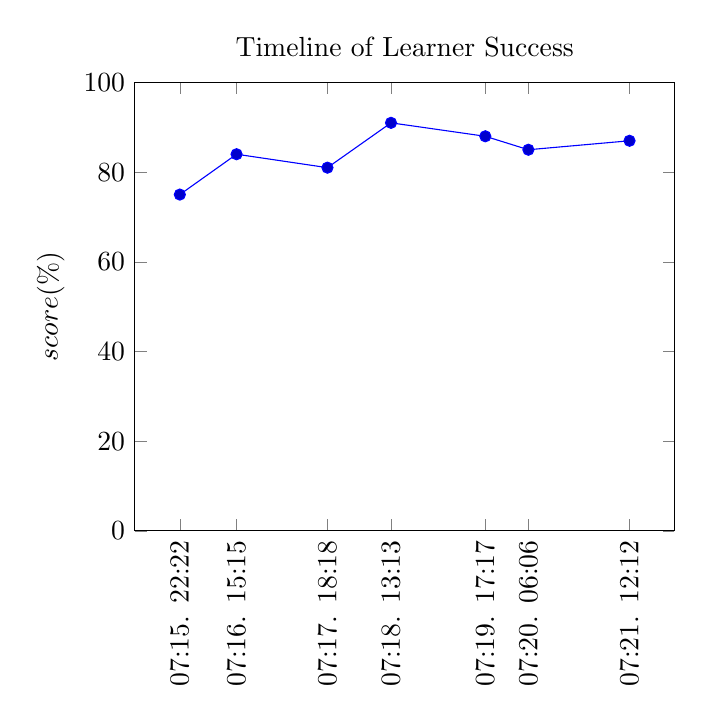
\begin{tikzpicture}
  \begin{axis}[
    title = Timeline of Learner Success,
    ylabel = $score(\%)$,
    ymin = 0,
    ymax = 100,
    date coordinates in=x,
    xtick=data,
    xticklabel style=
    {rotate=90,anchor=near xticklabel},
    xticklabel=\month:\day. \hour:\minute,]
    \addplot coordinates {
      (2018-07-15 22:22, 75.0)
      (2018-07-16 15:15, 84.0)
      (2018-07-17 18:18, 81.0)
      (2018-07-18 13:13, 91.0)
      (2018-07-19 17:17, 88.0)
      (2018-07-20 06:06, 85.0)
      (2018-07-21 12:12, 87.0)
    };
  \end{axis}
\end{tikzpicture}

\subsection{Prototype Improvement Suggestions}
Additional features may be implemented on top of this base
specification but they would require adding aditional values to each
subarray returned by the algorithm. These additional values can be
retrieved via (1) performing metadata lookup within or independently of the
algorithm (2) by utilizing additional xAPI statement paramters and/or (3) by
performing additional computations. The following examples assume the
metadata is contained within each statement available to the algorithm.
\begin{itemize}
\item A tooltip containing the name of an activity when hovering
  over a specific point on the chart
  \begin{itemize}
    \item this would require utilizing $\$.object.definition.name$
  \end{itemize}
\item A tooltip containing the device on which the activity was experienced
  \begin{itemize}
    \item this would require utilizing $\$.context.platform$
  \end{itemize}
\item A tooltip containing the instructor associated with a
  particular data point
  \begin{itemize}
    \item this would require utilizing $\$.context.instructor$
  \end{itemize}
\end{itemize}

\section{Which Assessment Questions are the Most Difficult}
As learners engage in a blended eLearning ecosystem, they will
experiecne teaching content as well as assessment content. Assessments
are designed to measure the effectiveness of learning content and help
measure learning. It is possible that certain assessment questions
do not accurately represent the concepts contained within teaching
material and this may be indicated by a majority of learners getting
the question wrong. It is also possible that the question accurately
represents the learning content but is just hard. The following
algorithm will identify these questions but will not be able to deduce
why learners answer them incorrectly.

\subsection{Ideal Statements}
In order to accurately determine which assessment questions are the
most dificult, there are a few requirements of the data produced by a
LRP. They are as follows:
\begin{itemize}
\item statements describing a learner answering a question must report
  if the learner got the question correct or incorrect via $\$.result.success$
\item if it is possible to get partial credit on a question, the amount
  of credit should be reported within the statement
  \begin{itemize}
  \item the credit earned by the learner should be reported within \\ $\$.result.score.raw$
  \item the minimum and maximum possible credit amount should be
    reported within $\$.result.score.min$ and $\$.result.score.max$
    respectively
  \end{itemize}
\item If it is possible to get partial credit on a question, it must
  still be reported if the learner reached the threshold of success
  via $\$.result.success$
\item Statements describing a learner answering a question should
  contain activities of the type $cmi.interaction$
\item activities must be uniquely and consistently identified across
  all statements
\item Statements describing a learner answering a question
  should\footnote{\label{verbIRI} it is possible to use another verb but if another is
      used, that will need to be accounted for in data retrieval} use
  the verb $http://adlnet.gov/expapi/verbs/answered$
\end{itemize}

\subsection{Input Data Retrieval}
How to query an LRS via a GET request to the Statements Resource
\footnote{\label{refMoreLink} See footnote 1.}
\footnote{\label{refnoZ} See footnote 2.}
\footnote{\label{refallTime} See footnote 3.}

\begin{lstlisting}[frame=single]
Verb = "verb=http://adlnet.gov/expapi/verbs/answered"

Since = "since=2018-07-20T12:08:47Z"

Until = "until=2018-07-21T12:08:47Z"

Base = "https://example.endpoint/statements?"

endpoint = Base + Verb + "&" + Since + "&" + Until

Auth = Hash generated from basic auth

S = curl -X GET -H "Authorization: Auth"
         -H "Content-Type: application/json"
         -H "X-Experience-API-Version: 1.0.3"
         Endpoint
\end{lstlisting}

\subsection{Statement Parameters to Utilize}
The statement parameter locations here are written in
\href{http://goessner.net/articles/JsonPath/}{JSONPath}. This notation
is also compatable with the xAPI Z notation due to the defined
hierarchy of components. Within the Z specifications, a variable name
will be used instead of the $\$$
\begin{itemize}
\item $\$.result.success$
\item $\$.object.id$
\end{itemize}

\subsection{2018 Pilot TLA Statement Problems}
The initial pilot test data supports this algorithm.
Given that the offical 2018 pilot test is scheduled to take place on July
27th, 2018, this section may require updates pending future data review.

\subsection{Summary}

\begin{enumerate}
\item Query an LRS via a \href{https://github.com/adlnet/xAPI-Spec/blob/master/xAPI-Communication.md#213-get-statements}{GET} request to the statements endpoint using the parameters verb, since and until
\item Filter the results to the set of statements where:
  \begin{itemize}
  \item $\$.result.success$ is false
  \end{itemize}
\item process the filtered data
  \begin{itemize}
  \item group by $\$.object.id$
  \item determine the count of each group
  \item create a collection of pairs = [$\$.object.id$, count]
  \end{itemize}
\end{enumerate}

\subsection{Formal Specification}

\subsubsection{Basic Types}

$INCORRECT$ :== $\{false\}$

\subsubsection{System State}

\begin{schema}{MostDifficultAssessmentQuestions}
  Statements \\
  S_{all} : \finset_1 \\
  S_{incorrect},S_{grouped},S_{processed} : \finset \\
  \where
  S_{all} = statements \\
  S_{incorrect} \subseteq S_{all} \\
  S_{grouped} = \{groups : \seq_1 statement\} \\
  S_{processed} = \{pair : (id , \nat)\}
\end{schema}
\begin{itemize}
\item The set $S_{all}$ is a non-empty, finite set and is the
  component $statements$
\item The sets $S_{incorrect}$, $S_{grouped}$ and $S_{processed}$ are all finite sets
\item the set $S_{incorrect}$ is a subset of $S_{all}$
\item the set $S_{grouped}$ is a finite set of objects $groups$ which
  are non-empty, finite sequences of the component $statement$
\item the set $S_{processed}$ is a finite set of pairs where each
  contains the component $id$ and a natural number
\end{itemize}

\subsubsection{Initial System State}

\begin{schema}{InitMostDifficultAssessmentQuestions}
  MostDifficultAssessmentQuestions \\
  \where
  S_{all} \not = \emptyset \\
  S_{incorrect} = \emptyset \\
  S_{grouped} = \emptyset \\
  S_{processed} = \emptyset
\end{schema}
\begin{itemize}
\item The set $S_{all}$ is a non-empty set
\item The sets $S_{incorrect}$ , $S_{grouped}$ and $S_{processed}$ are all initially empty
\end{itemize}

\subsubsection{Filter for Incorrect}

\begin{schema}{Incorrect}
  Statement \\
  incorrect : STATEMENT \pfun \finset \\
  s? : STATEMENT \\
  s! : \finset \\
  \where
  s? = statement \\
  s! = incorrect(s?) \\
  incorrect(s?) = \IF s?.result.success : INCORRECT \\\t4 \THEN s! =
  s? \\\t4 \ELSE s! = \emptyset
\end{schema}
\begin{itemize}
\item the schema $Incorrect$ introduces the function $incorrect$ which
  takes in the variable $s?$ and returns the variable $s!$
\item the variable $s?$ is the component $statement$
\item $s!$ is equal to $s?$ if $\$.result.success$ is of the type
  $INCORRECT$ otherwise $s!$ is an empty set
\end{itemize}

\begin{schema}{FilterForIncorrect}
  \Delta MostDifficultAssessmentQuestions \\
  Incorrect \\
  incorrects : \finset
  \where
  incorrects = S_{all} \\
  incorrects' = \{s : STATEMENT \,|\, incorrect(s) \not = \emptyset\} \\
  S_{incorrect}' = S_{incorrect} \cup incorrects'
\end{schema}
\begin{itemize}
\item the set $incorrects$ is the set $S_{all}$
\item The set $incorrects'$ contains elements $s$ of type $STATEMENT$
  where $incorrect(s)$ is not an empty set
\item The updated set $S_{incorrect}'$ is the union of the previous
  state of $S_{incorrect}$ and $incorrects'$
\end{itemize}

\subsubsection{Processes Results}

\begin{schema}{GroupByActivityId}
  Statements \\
  g? : \finset \\
  g! : \finset \\
  group : \finset \fun \finset
  \where
  g? = statements \implies \{g : statement\} \\
  g! = group(g?) \\
  g! = \{groups : \seq_1 statement \,|\, \\ \t1
  \LET \seq_1 statement_{i}..statement_{j} == \seq_1 s_{i}..s_{j} @ \\\t1
  \forall s : s_{i}..s_{j} @ s_{i}.object.id = s_{j}.object.id\} \\
\end{schema}
\begin{itemize}
  \item The schema $GroupByActivityId$ introduces the function $group$
    which has the input of $g?$ and the output of $g!$
  \item The input variable $g?$ is the component $statements$ which implies
    its a set of objects $g$ which are each a $statement$
  \item the output variable $g!$ is a set of objects $groups$ which
    are each a non-empty, finite sequence of $statement$ where each
    member of the sequence $s_{i}..s_{j}$ has identical object ids.
\end{itemize}

\begin{schema}{CountPerGroup}
  Statement \\
  c? : \seq_1 statement \\
  c! : \nat \\
  count : \seq_1 statement \fun \nat
  \where
  c! = count(c?) \\
  c! \geq 1 \\
  count(c?) = \forall c? : c?_{i}..c?_{j} @ i,j : \nat \land i
  = 0 \land i = j \lor i \not = j @  \\\t3 \exists_1 \, c! : \nat @  c! =
  j + 1
\end{schema}
\begin{itemize}
  \item The schema $CountPerGroup$ introduces the function $count$
    which has the input of $c?$ and the output of $c!$
  \item The input variable $c?$ is a non-empty, finite sequence in which each element is
    a $statement$
  \item The function $count$ reads: for all elements within the
    sequence $c?_{i}..c?_{j}$, $i$ and $j$ are natural numbers, $i$ is
    equal to zero and may or may not be equal to $j$ such that there
    exits a number $c!$ which is equal to $j + 1$
\end{itemize}

\begin{schema}{AggregateQuestionStatements}
  \Delta MostDifficultAssessmentQuestions \\
  FilterForIncorrect \\
  GroupByActivityId \\
  CountPerGroup \\
  grouped, processed : \finset \\
  \where
  grouped = \emptyset \\
  grouped' = group(S_{incorrect}) \\
  S_{grouped}' = S_{grouped} \cup grouped' \\
  processed = S_{grouped}' \\
  processed' = \{p : (id, \nat) \,|\, \\\t3 \LET
  \{processed_{i}..processed_{j}\} == \{g_{i}..g_{j}\} @ \\\t3
  \forall g : g_{i}..g_{j} @ \exists \,\, p_{i}..p_{j} @ \\\t3
  first~p_{i} = head~g_{i}.object.id \, \land second~p_{i} =
  count(g_{i}) \\\t3 first~p_{j} = head g_{j}.object.id \land
  second~p_{j} = count(g_{j})\} \\
  S_{processed}' = S_{processed} \cup processed'
\end{schema}
\begin{itemize}
\item The schema $AggregateQuestionStatements$ introduces the variables
  $grouped$ and $processed$
\item $grouped$ starts as an empty set but then becomes $grouped'$
  which is the output of applying the function $group$ to the set of statements
  $S_{incorrect}$ created by the opperation $FilterForIncorrect$
\item $grouped'$ is a set of sequences. The elements of those
  sequences are statements which all have the same $statement.object.id$
\item The set $S_{grouped}$ is updated to the set $S_{grouped}'$ which
  is the union of $S_{grouped}$ and $grouped'$
\item the variable $processed$ is initialized to be $S_{grouped}'$
\item the variable $processed$ is updated to be the variable
  $processed'$ which is a set of objects $p$ which are ordered pairs
  of the component $id$ and a natural number. $p$ is defined as:
  \begin{itemize}
  \item for all sequences $g_{i}..g_{j}$ within the set $processed$,
    there exists ordered pairs $p_{i}..p_{j}$ such that:
    \begin{itemize}
    \item the first element of $p_{i}$ is equal to the $object.id$ of the first
      statement within the sequence $g_{i}$.
    \item The second element of $p_{i}$ is equal to the value returned
      when $g_{i}$ is passed to the function $count$.
    \item The first element of $p_{j}$ is equal to the $object.id$ of the
      first statement within the sequence $g_{j}$.
    \item the second element of $p_{j}$ is equal to the value returned
      when $g_{j}$ is passed to the function $count$
    \end{itemize}
  \end{itemize}
  \item The set $S_{processed}'$ is the union of the sets
    $S_{processed}$ and $processed'$
\end{itemize}

\subsubsection{Sequence of Operations}

$ProcessedQuestions \defs FilterForIncorrect \semi AggregateQuestionStatements$
\begin{itemize}
\item The schema $ProcessedQuestions$ is the sequential composition
  of operation schemas $FilterForIncorrect$ and
  $AggregateQuestionStatements$
\item $FilterForIncorrect$ happens before $AggregateQuestionStatements$
\end{itemize}

\subsubsection{Return}

\begin{schema}{ReturnAggregate}
  \Xi MostDifficultAssessmentQuestions \\
  ProcessedQuestions \\
  S_{processed}! : \finset
  \where
  S_{processed}! = S_{processed}
\end{schema}
\begin{itemize}
\item The returned variable $S_{processed}!$ is equal to the current
  state of variable $S_{processed}$ after the operations
  $FilterForIncorrect$ and \\ $AggregateQuestionStatements$
\end{itemize}

\subsection{Pseudocode}

\begin{algorithm}[H]

  \SetAlgoLined

  \KwIn{$S_{all}$, display-n}
  \KwResult{display}
  init id-to-count := [] \\
  init display := [] \\
  \While{$S_{all}$ is not empty} {
    for each statement $s$ in $S_{all}$ \\
    \eIf{$s.result.success$ = $INCORRECT$}
    {
      add $s$ to $S_{incorrect}$ \\
      remove $s$ from $S_{all}$ \\
      recur
    }
    {
      remove $s$ from $S_{all}$ \\
      recur
    }}
  \While {$S_{incorrect}$ is not empty} {
    for {each statement $si$ in $S_{incorrect}$} \\
    \t1 let $si.object.id$ = $id$ \\
    \eIf{id-to-count is empty}
    { concat id-to-count [$id$ , 1] \\
      remove $si$ from $S_{incorrect}$\\
      recur;}
    {
      \eIf{id-to-count contains [$id$ , \#]}
      { add one to \# \\
        remove $si$ from $S_{incorrect}$ \\
        recur}
    { concat id-to-count [$id$ , 1] \\
      remove $si$ from $S_{incorrect}$\\
      recur}
    }
  }
  Sort id-to-count by second value of each subarray (\#) \\
  take first display-n subarrays from id-to-count and concat them into display
  \caption{Most Difficult Assessment Questions}
\end{algorithm}
\begin{itemize}
\item The Z schemas are used within this pseudocode
\item The return value display is an array of display-n arrays, each containing an
   object id and a number representing the number of times it showed up.
\end{itemize}

\subsection{JSON Schema}

\begin{lstlisting}[style=json]
{"type":"array",
   "items":{"type":"array",
      "items":[{"type":"string"}, {"type":"number"}]}
}
\end{lstlisting}

\subsection{Visualization Description}
The Most Difficult Assessment Questions visualization will be a bar
chart where the domain is statement id and the range is a
number. Every subarray within the array returned by the algorithm will
contribute to the bar chart. The pseudocode specifies an input
paramter display-n which controls how many activitys will be displayed
within the visualization.

\subsection{Visualization prototype}

\pgfplotstabletypeset[string type]

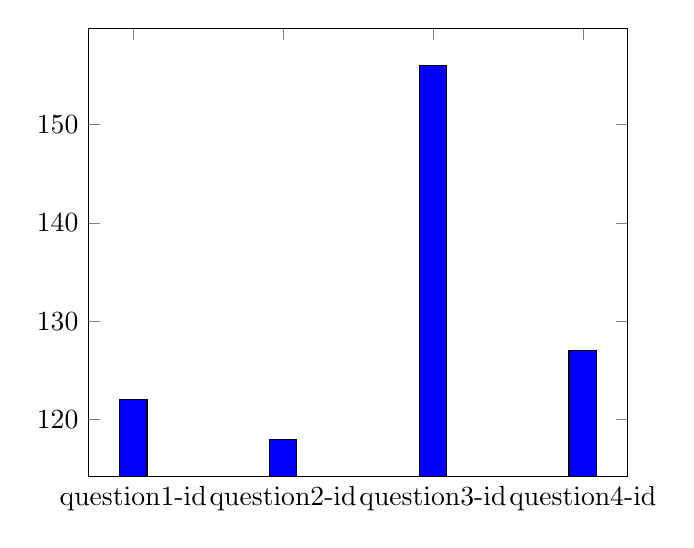
\begin{tikzpicture}
\begin{axis}[
    symbolic x coords={question1-id,question2-id,question3-id,question4-id},
    xtick=data]
    \addplot[ybar,fill=blue] coordinates {
        (question1-id,122)
        (question2-id,118)
        (question3-id,156)
        (question4-id,127)
    };
\end{axis}
\end{tikzpicture}

\subsection{Prototype Improvement Suggestions}
Additional features may be implemented on top of this base
specification but they would require adding aditional values to each
subarray returned by the algorithm. These additional values can be
retrieved via (1) performing metadata lookup within or independently of the
algorithm (2) by utilizing additional xAPI statement paramters and/or (3) by
performing additional computations. The following examples assume the
metadata is contained within each statement available to the algorithm.


\begin{itemize}
\item Use the name of the activity for the x-axis label instead of
  its id.
  \begin{itemize}
  \item $\$.object.definition.name$
  \item grouping of statements should still happen by
    $\$.object.id$ to ensure an accurate count
  \end{itemize}
\item a tooltip containing contextual information about the question
  such as:
  \begin{itemize}
  \item The question text
    \begin{itemize}
    \item $\$.object.definition.description$
    \end{itemize}
  \item Interaction Type
    \begin{itemize}
      \item $\$.object.definition$ which specifies interaction properties
    \end{itemize}
  \item Answer choices
    \begin{itemize}
      \item $\$.object.definition$ which specifies interaction properties
    \end{itemize}
  \item Correct answer
    \begin{itemize}
      \item $\$.object.definition$ which specifies interaction properties
    \end{itemize}
  \item Most popular incorrect answer
    \begin{itemize}
      \item This would require an extra step of processing to be added to
      the algorithm and that all statements utilize interaction
      properties within $\$.object.definition$
    \end{itemize}
  \item average partial credit earned (if applicable)
    \begin{itemize}
    \item $\$.result.score.scaled$
    \item The one potential issue with using scaled score is the
      calculation of scaled is not stricly defined by the xAPI
      specification and thus the average scaled score may not be
      comparable across questions.
    \item if $\$.result.score.raw$ , $\$.result.score.min$ and
      $\$.result.score.max$ are reported for all questions, it becomes
      possible to reliably compare across questions.
    \end{itemize}
  \item average number of re-attempts
    \begin{itemize}
      \item this would require additional steps of processing so that
        $\$.actor$ is considered as well
      \item due to the problem of actor unification, ie the same
        person being identified differently across statements, this
        metric may not be accurate
      \end{itemize}
    \item average time spent on the question
      \begin{itemize}
      \item $\$.result.duration$
      \item this would require additional steps of processing to
        extract the duration and average it.
      \end{itemize}
    \end{itemize}
  \item a tooltip containing contextual information about the course
    and/or assessment the question was within
    \begin{itemize}
    \item the instructor for the course
      \begin{itemize}
      \item $\$.context.instructor$
      \end{itemize}
    \item competency associated with the question
      \begin{itemize}
      \item $\$.context.contextActivities$
      \end{itemize}
    \item metadata about the learning content associated with the
      question such as average time spent engaging with associated
      learning content before attempting the question
    \item this would require additional steps of processing to
      retrieve metadata about the content and its usage
      \begin{itemize}
      \item $\$.context.contextActivities$
      \end{itemize}
    \end{itemize}
\end{itemize}

\end{document}
